\documentclass[11pt,a4paper]{article}
\usepackage[T1]{fontenc}
\usepackage[utf8]{inputenc}
\usepackage[french]{babel}
\usepackage{lmodern}
\usepackage{amsmath,amssymb}
\usepackage[margin=2.5cm]{geometry}
\usepackage{booktabs}
\usepackage{graphicx}
\usepackage{enumitem}
\usepackage{xcolor}
\usepackage{hyperref}
\hypersetup{colorlinks=true,linkcolor=blue!50!black}

\newcommand{\NW}{\mathrm{NW}}
\newcommand{\E}{\mathbb{E}}
\newcommand{\code}[1]{\texttt{#1}}

\title{Validation expérimentale du modèle M2\\
\large Protocole §6 du document de conception, outils corrigés\\
(workspace \code{m2\_fable})}
\author{Agent de réplication (workspace \code{m2\_fable})}
\date{3 juillet 2026}

\begin{document}
\maketitle

\begin{abstract}
Nous validons l'implémentation M2 sur le protocole §6 du document de
conception, avec les outils statistiques corrigés (MLE tronqués, cf. rapport
d'implémentation) et des ablations que le rapport ne prévoyait qu'en recours.
Bilan par cible : \textbf{population bornée endogènement : confirmé} (et,
fait nouveau, le crédit n'y est pour rien) ; \textbf{queue d'exposant stable :
confirmé et étendu} ($\alpha \approx 2{,}7$ stationnaire sur $6000$ pas, là
où le WIP dérivait de $5{,}4$ à $3{,}1$) — mais l'ablation sans crédit produit
\emph{exactement la même queue} : la stabilité vient de la démographie
(GBM $\times$ mortalité $\times$ mélange d'âges, mécanisme à la Reed), pas de
la boucle crédit-cascades ; de plus le test LR corrigé préfère
systématiquement la log-normale tronquée à la loi de puissance ;
\textbf{classes dynamiques : confirmé} au-delà des seuils demandés ;
\textbf{corps exponentiel : réfuté} (Fisk gagne partout ; le drift mesuré du
corps est ascendant, incompatible avec le mécanisme [YR] postulé), avec la
nuance importante que le corps est \emph{quasi} exponentiel (QQ-plot
linéaire, $\mathrm{med}/\mathrm{mean} = 0{,}69$--$0{,}70 \approx \ln 2$).
Enfin, la règle M2 de transfert des créances au prorata rend le carnet de
contrats non stationnaire (jusqu'à $2,6 \cdot 10^6$ contrats sur une case de
la grille), et la convention « moyenne géométrique des taux » se révèle
constitutive : en moyenne arithmétique, le marché du crédit meurt.
\end{abstract}

\tableofcontents

\section{Dispositif}

\paragraph{Runs.} Baseline (config du rapport : $\alpha=1$, $\delta=0{,}05$,
$k=6$, $\sigma=0{,}25$, $\lambda=10$, $w_0=30$, $d_0=28$, $N(0)=0$, $T=2000$),
seeds $\{0,1,2\}$. Ablations (2 seeds chacune) : \code{proto\_e7c}
(créances de la faillie annulées, comme le prototype du rapport),
\code{destroy} (capital résiduel détruit au lieu de distribué),
\code{nocredit} (modèle nul sans marché), \code{arith} (taux en moyenne
arithmétique), \code{lam30} ($\lambda = 30$). Runs longs $T = 6000$
(\code{nocredit} et \code{proto\_e7c}, 2 seeds). Grille §6.5 :
$\sigma \in \{0{,}15 ; 0{,}25 ; 0{,}35\} \times \varepsilon_0/w_0 \in
\{0{,}05 ; 0{,}25 ; 0{,}5\} \times k \in \{3, 6\}$, plus $k \in \{2, 4\}$ à la
baseline.

\paragraph{Mesures.} Fenêtres $[500,1000)$, $[1000,1500)$, $[1500,2000)$
(runs longs : 11 fenêtres de 500 pas), pools d'instantanés tous les 50 pas
\emph{au sein d'une fenêtre et d'un seed}, jamais entre seeds. Corps : MLE
\emph{tronqué} exponentielle/gamma/log-normale/Fisk sur les 95\,\%
inférieurs, AIC. Queue : CSN ($x_{\min}$ par KS, MLE), exposants comparés à
$x_{\min}$ commun (médiane des fenêtres) avec IC bootstrap à 95\,\%
(200 rééchantillonnages), LR de Vuong contre la log-normale \emph{tronquée
en $x_{\min}$} (correction du biais pro-Pareto du test historique, rapport
d'implémentation §4.3). Conventions : $\alpha$ désigne l'exposant de la
densité, $p(x) \propto x^{-\alpha}$ ($\alpha = 1 + \mu$ au sens [BM]).

\section{Cible 1 : population bornée endogènement — CONFIRMÉ}

$N(t)$ plat hors transitoire pour la baseline : moyenne
$1591/1639/1655$ (seeds 0/1/2) sur $[800, 2000]$, pente relative
$+0{,}05$ à $+0{,}09$ pour 1000 pas (résiduel de transitoire, décroissant).
Faillites $\approx$ naissances ($9{,}6$ contre $10$ par pas). Extensivité
en $\lambda$ : $N^*/\lambda = 166{,}3$ ($\lambda = 10$) contre $166{,}4$
($\lambda = 30$) — remarquablement exact, conforme à $N^* = \lambda\,
\E[\text{vie}]$ avec $\E[\text{vie}] \approx 166$ pas.

\textbf{Résultat non prévu par le rapport} : le modèle nul \code{nocredit}
est lui aussi borné ($N^* \approx 1851$--$1939$, $+12$\,\% par rapport à la
baseline). Le bornage est donc entièrement porté par le trio
$\{\sigma, d_0, \text{extraction}\}$ : le crédit n'est pas nécessaire (il
\emph{augmente} légèrement la mortalité, d'où le $N^*$ plus faible avec
crédit). L'affirmation du rapport était prudente sur ce point ([E6] montrait
déjà un monde borné à crédit mort) ; la confirmation est nette.

\begin{center}
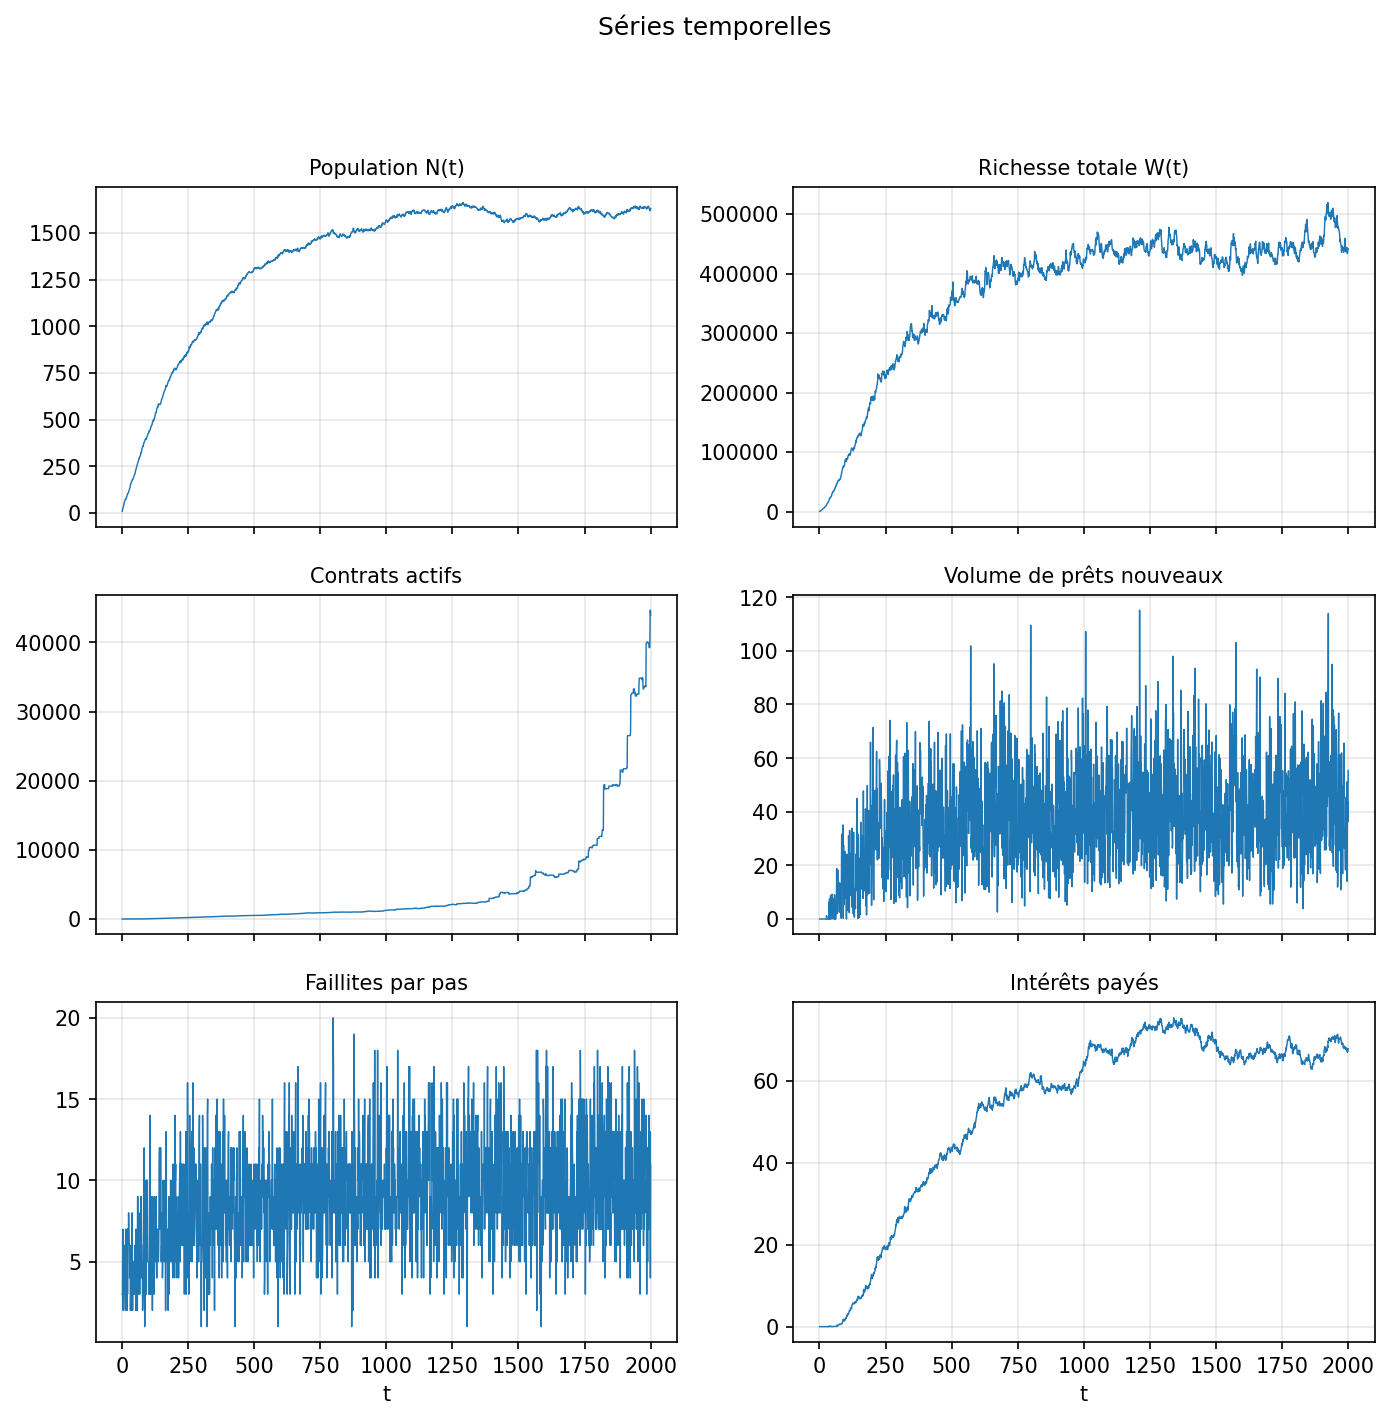
\includegraphics[width=0.95\textwidth]{figures/timeseries.png}
\end{center}

\section{Cible 2 : queue de Pareto stable — CONFIRMÉ, MAIS…}
\label{sec:queue}

\subsection{Stabilité : oui, et mieux que demandé}
Baseline, $\NW$, exposant à $x_{\min}$ commun par seed (IC bootstrap 95\,\%) :

\begin{center}
\small
\begin{tabular}{lccc}
\toprule
seed & $[500,1000)$ & $[1000,1500)$ & $[1500,2000)$\\
\midrule
0 & $2{,}67$ $[2{,}59 ; 2{,}73]$ & $2{,}74$ $[2{,}67 ; 2{,}81]$ & $2{,}79$ $[2{,}72 ; 2{,}87]$\\
1 & $2{,}74$ $[2{,}65 ; 2{,}82]$ & $2{,}77$ $[2{,}70 ; 2{,}85]$ & $2{,}78$ $[2{,}71 ; 2{,}85]$\\
2 & $2{,}60$ $[2{,}55 ; 2{,}65]$ & $2{,}56$ $[2{,}52 ; 2{,}63]$ & $2{,}63$ $[2{,}58 ; 2{,}69]$\\
\bottomrule
\end{tabular}
\end{center}

Dérive intra-seed $\le +0{,}12$ (seed 0, marginalement hors IC ; seeds 1--2
stables), inter-seed $\pm 0{,}1$. Les runs longs ($T = 6000$, 11 fenêtres,
figure ci-dessous) ne montrent \emph{aucune} dérive :
$\alpha \in [2{,}65 ; 2{,}81]$, fluctuations dans les IC. C'est exactement le
critère que le WIP ratait ($5{,}4 \to 3{,}1$) ; les valeurs répliquent
[E7c] ($2{,}70/2{,}79/2{,}84$) malgré une règle de faillite différente.

\begin{center}
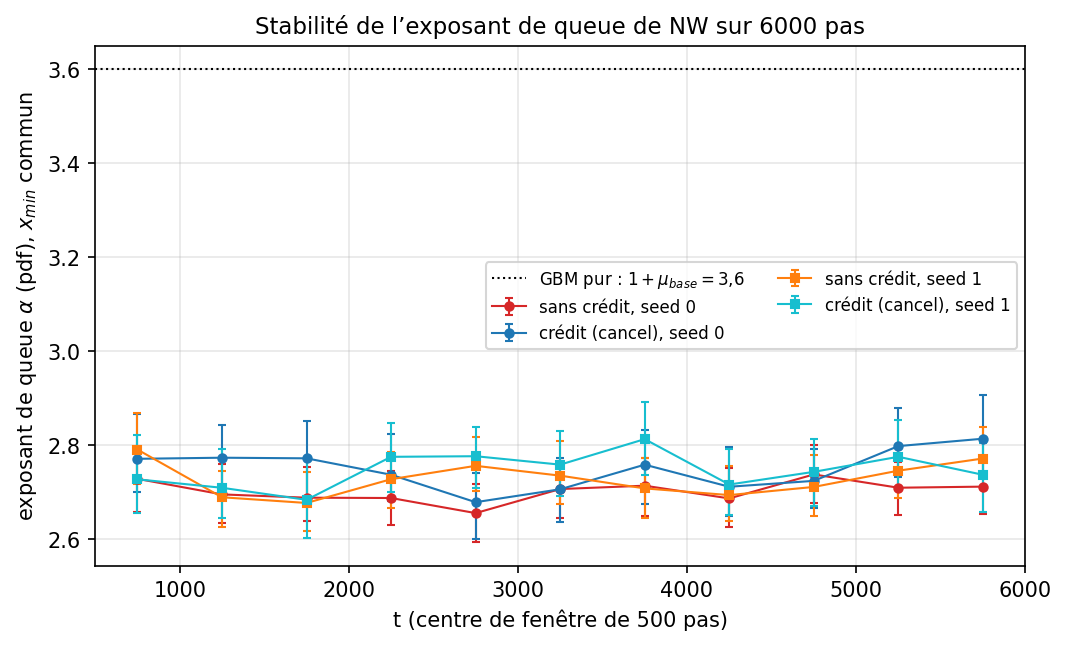
\includegraphics[width=0.9\textwidth]{figures/alpha_drift_long.png}
\end{center}

\subsection{…l'attribution causale du rapport est réfutée}
La figure ci-dessus contient le résultat le plus important de cette
validation : les runs \code{nocredit} (rouge/orange) ont \emph{la même
queue, aussi stable, au même exposant} que les runs avec crédit
(bleu/cyan). À $T = 2000$ comme à $T = 6000$, aucune mesure
distributionnelle ne distingue le modèle complet du modèle nul : exposant
($2{,}6$--$2{,}8$ contre $2{,}6$--$2{,}8$), corps (Fisk contre Fisk),
$\mathrm{med}/\mathrm{mean}$ ($0{,}69$ contre $0{,}69$), renouvellement du
top décile ($\approx 90$\,\% de nés récents dans les deux cas).

Interprétation mécanistique : la queue stationnaire vient du mélange
démographique — chaque entité suit un GBM (choc $\sigma$) rappelé par
l'extraction et tué au plancher $\NW = 0$ ; une population d'âges
exponentiellement mélangés de trajectoires log-normales produit une queue en
loi de puissance stationnaire (mécanisme de type Reed / double-Pareto). La
boucle « crédit $\to$ concentration $\to$ cascades $\to$ $\mu$ » (H2, §3.4 du
rapport) n'est pas nécessaire pour la stabilité observée, et rien ne montre
qu'elle agisse : cf. \S\ref{sec:soc}.

Deux repères quantitatifs affaiblissent encore H2 : (i) l'exposant mesuré
($\approx 2{,}7$) est loin du repère Kesten sans crédit du rapport
($1 + \mu_{\mathrm{base}} = 3{,}6$ pour $\delta = 0{,}05$,
$\sigma = 0{,}25$) — or c'est le modèle \emph{sans crédit} qui le réalise :
la dérivation §3.3 du rapport ne décrit donc pas le mécanisme dominant de sa
propre queue (le rappel $\sqrt{w}$ et le plancher $\NW$, ignorés par le
calcul de $\mu_{\mathrm{base}}$, dominent) ; (ii) $\lambda = 30$ donne le
même exposant ($2{,}69/2{,}71/2{,}68$), ce qui est cohérent avec la
prédiction (ii) de §3.4… mais aussi avec n'importe quel mécanisme
démographique extensif.

\subsection{Loi de puissance contre log-normale : le verdict s'inverse}
Avec le LR corrigé (log-normale tronquée), la loi de puissance ne gagne
\emph{jamais} : sur $\NW$, baseline, $R < 0$ dans 9 fenêtres sur 9, dont 7
significatives ($p < 0{,}05$). Idem sur les runs longs (22 fenêtres, $R < 0$
partout). Le LR \emph{naïf} (celui du script historique) donne au contraire
$R \gg 0$, $p \approx 0$ partout — y compris, test de contrôle, sur des
données log-normales pures. \textbf{La « préférence pour la loi de
puissance » de [E7c] était un artefact du test.} La description la plus
parcimonieuse de la queue M2 est une log-normale tronquée, dont l'exposant
\emph{effectif} est stationnaire par mélange démographique. Notons que la
distinction a une portée limitée (une log-normale tronquée à grand $\sigma$
et une Pareto sont quasi indiscernables) ; l'important est la stationnarité,
qui est acquise.

\section{Cible 3 : corps exponentiel — RÉFUTÉ (mais quasi exponentiel)}
\label{sec:corps}

\subsection{Ajustements}
Sur $\NW$ (baseline, 9 fenêtres $\times$ seeds, MLE tronqué) : Fisk gagne
partout, $\Delta\mathrm{AIC}_{\exp} = 500$--$780$ sur $n \approx 15\,000$
(pools) et $43$--$61$ sur $n \approx 1500$ (instantanés uniques — l'écart
n'est donc \emph{pas} un artefact de pooling). Sur le revenu et $w$ :
log-normale, avec $\mathrm{med}/\mathrm{mean}(\text{revenu}) = 0{,}92$
(corps en bosse, franchement non exponentiel). Critère §6.1 du rapport
(l'exponentielle gagne ou $\Delta\mathrm{AIC} \le 2$) : \textbf{échec} sur
les trois variables, tous seeds, toutes fenêtres.

\subsection{La nuance : quasi-exponentialité de $\NW$}
$\mathrm{med}/\mathrm{mean}$ du corps de $\NW$ : $0{,}685$--$0{,}706$
($\ln 2 = 0{,}693$), stable sur 22 fenêtres de runs longs ; QQ-plot
exponentiel linéaire jusqu'au dernier vingtile ; histogramme décroissant dès
le premier bin (mode en 0). L'écart à l'exponentielle est réel
(AIC, $\approx 0{,}03$ de log-vraisemblance par point) mais petit. La forme
[BM] éq.~(7) (coupure basse $e^{-(\mu-1)/X}$, c'est-à-dire une
inverse-gamma), alternative prévue par X1.4 du rapport, a été testée en MLE
tronqué sur les mêmes pools : elle est \emph{massivement rejetée}
($\Delta\mathrm{AIC} = +4236$ contre Fisk, ajustement dégénéré) — le corps
de M2 n'est ni [YR] ni [BM]. Classement complet (pool $[1500,2000)$,
seed 0) : Fisk $\prec$ gamma ($+344$) $\prec$ log-normale ($+489$) $\prec$
exponentielle ($+566$) $\prec$ inverse-gamma ($+4236$). La photographie
honnête : \emph{corps exponentiel à l'œil, Fisk au microscope}.

\begin{center}
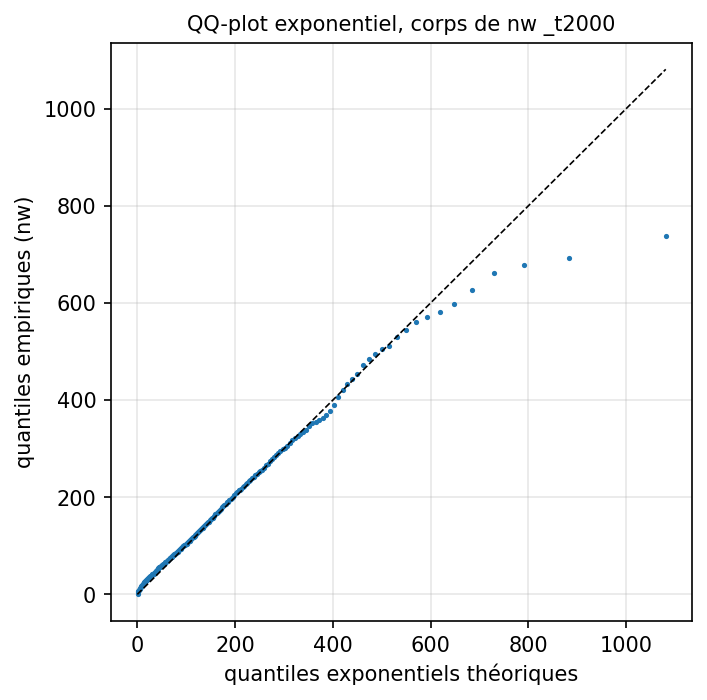
\includegraphics[width=0.55\textwidth]{figures/qq_expon_nw_t2000.png}
\end{center}

\subsection{Le mécanisme postulé est contredit}
Test mécanistique §6.1 (incréments 1 pas de $\NW$, entités du corps,
fenêtre fixe $[0, q_{70}]$, snapshots denses $t \in [1500, 1520]$) :
le drift mesuré est \emph{ascendant} ($\E[\Delta\NW] = +4{,}15 \pm 0{,}1$
par pas, cohérent sur 3 seeds et toutes variantes), soit $A_0 = -4{,}15 < 0$
au sens [YR], avec $B_0 \approx 600$. Le corps exponentiel de [YR] éq.~(7)
exige $A_0 > 0$ (drift vers le plancher compensé par la diffusion). Ici le
corps est un \emph{régime de transport} : les entités y montent en moyenne
(vers le point fixe autarcique), la stationnarité étant assurée par la
réinjection à $\varepsilon_0$ et la mortalité, pas par un équilibre
drift-diffusion. $T = B_0/A_0$ n'est pas défini (signe) ; l'échelle mesurée
du corps ($\approx 190$) n'est pas $B_0/A_0$. \textbf{H1 est réfutée dans son
mécanisme, pas seulement dans sa forme.} Réserve : les incréments excluent
les entités mortes dans l'intervalle (biais de survie) ; l'ordre de grandeur
du flux de décès ($0{,}6$\,\% par pas, incréments négatifs de l'ordre de
$-100$) ne suffit pas à inverser le signe.

\section{Cible 4 : classes dynamiques, pas démographiques — CONFIRMÉ}

\begin{itemize}[nosep]
\item $\mathrm{corr}(\text{âge}, \log \NW) = 0{,}09$--$0{,}15$ (seuil du
  rapport : $< 0{,}85$ ; WIP : $0{,}88$--$0{,}95$) ;
\item top décile de $\NW$ entre $t=1000$ et $t=2000$ : survie
  $11$--$17$\,\% (sur 1000 pas), persistance dans le top $0{,}6$--$3{,}2$\,\%,
  fraction du top de $t=2000$ née après $t=1000$ : $90$--$95$\,\%
  (critère : $\ge 20$\,\%), dates de naissance étalées
  ($q_{10}$--$q_{90} \approx 1000$--$1915$) ;
\item queue présente à âge contrôlé sur $\NW$ (tranches $[50,150)$ et
  $[150,400)$ : $\alpha \approx 2{,}1$--$2{,}7$) ;
\item distribution d'âges continue, sans trou ($q_{10}/q_{50}/q_{90}
  = 33/261/873$).
\end{itemize}

Nuance instructive : la mortalité \emph{instantanée} du top décile est
nulle (personne ne meurt riche) — on quitte d'abord le top par chocs et
charges, puis on meurt pauvre. Le renouvellement massif ci-dessus montre que
cette descente est rapide ($\E[\text{séjour au top}] \ll 1000$ pas). La
formulation du critère 6.4 du rapport (« mortalité du top $> 0$ ») était
mal posée ; le renouvellement est la bonne mesure, et il est excellent.

\begin{center}
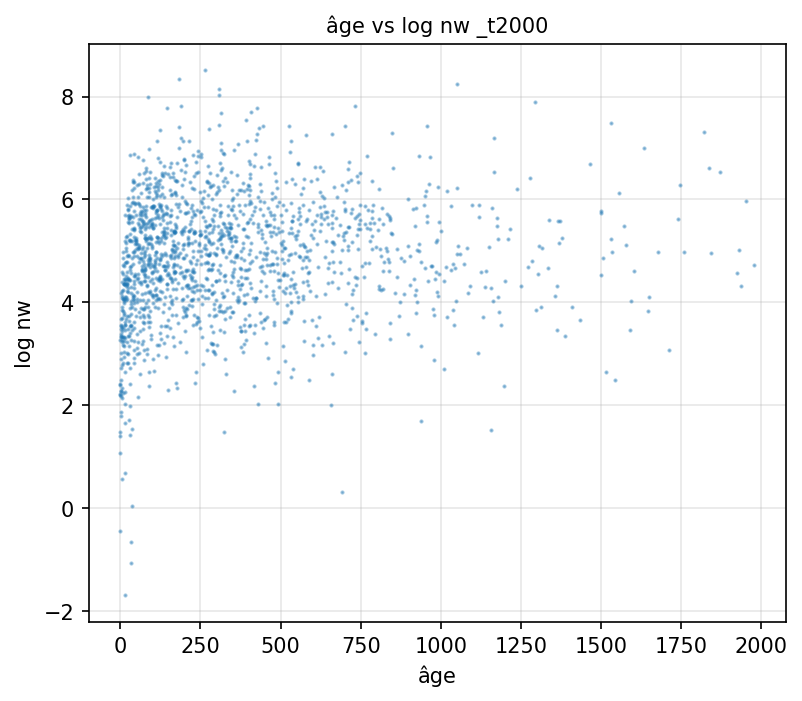
\includegraphics[width=0.48\textwidth]{figures/age_lognw_t2000.png}
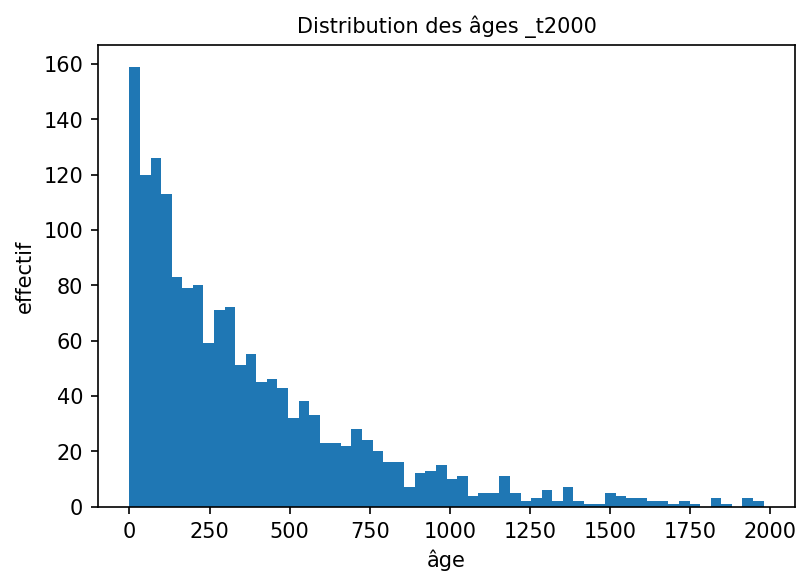
\includegraphics[width=0.44\textwidth]{figures/ages_t2000.png}
\end{center}

\section{Diagnostics SOC — le mécanisme H2 est invisible}
\label{sec:soc}

\begin{itemize}[nosep]
\item \textbf{Tailles de cascade} : faillites par pas $\approx$
  Poisson($\lambda$) étroit (moyenne $9{,}6$, max $20$--$21$, $p_{99} = 17$
  sur 1500 pas $\times$ 3 seeds). Aucune queue lourde à $k = 6$. Les
  « cascades » sont des coïncidences de mortalité individuelle, pas des
  avalanches : le réseau ne propage pas.
\item \textbf{Concentration $\to$ cascades} : la part du top décile des
  créances est élevée ($82$\,\%) mais sa corrélation avec les faillites des
  50 pas suivants est nulle ($-0{,}03$ à $-0{,}11$).
\item \textbf{Rôle causal du crédit} : nul sur la distribution
  (\S\ref{sec:queue}), léger sur la démographie ($+10$\,\% de mortalité).
\end{itemize}

La boucle auto-critique de §3.4 du rapport (levier $\leftrightarrow$
cascades) n'a donc \emph{aucun support empirique} dans le régime baseline.
Le balayage en $k$ et la grille (\S\ref{sec:grille}) précisent si un régime
SOC existe ailleurs.

\begin{center}
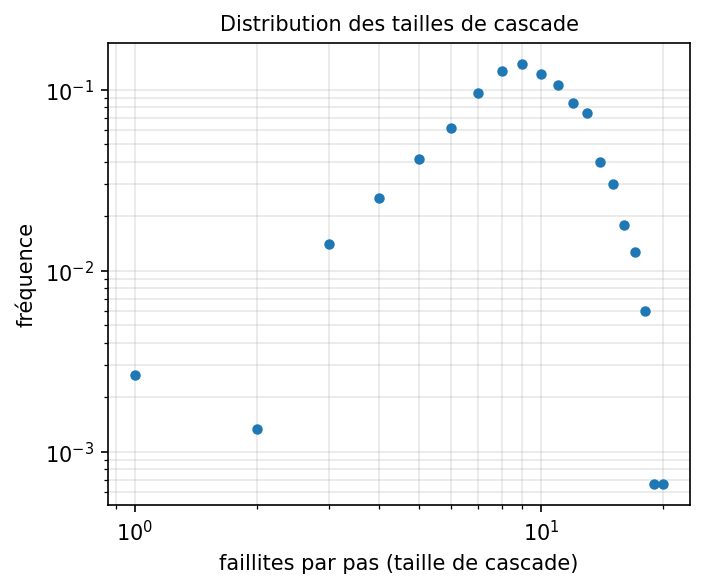
\includegraphics[width=0.5\textwidth]{figures/cascades.png}
\end{center}

\section{Robustesse : grille §6.5, balayage $k$, conventions}
\label{sec:grille}

\subsection{Fenêtre de naissance : les bornes mordent comme prévu}
Toute la ligne $\sigma = 0{,}15$ de la grille sort du régime cible : la
mortalité s'effondre (0 à 1 faillite par pas), la population atteint
$15\,500$--$20\,000$ à $T = 2000$ et croît encore — conforme à la borne
basse $w_0 \gtrsim 1/(\sigma+\delta)^2 = 25$ ($w_0 = 30$, marginal) et au
diagnostic [E7a] du rapport. C'est une \emph{prédiction confirmée} du
rapport, mais aussi la confirmation que la forme cible n'existe que dans une
fenêtre de paramètres calée : hors fenêtre, pas de réglage progressif mais
un changement de régime (mortalité nulle).

\subsection{Prolifération des contrats hors baseline}
La case $(\sigma = 0{,}25, \varepsilon_0/w_0 = 0{,}25, k = 6)$ finit avec
$2{,}58 \cdot 10^6$ contrats actifs (contre $\approx 600$ pour la variante
\code{cancel} à la baseline) : la règle de transfert au prorata (§2.2
phase 7 du rapport) est non stationnaire et devient pathologique dès que la
démographie ralentit. Toute exploitation future de M2 devra soit adopter
\code{cancel} (qui ne change aucune conclusion distributionnelle, cf.
ablation), soit consolider les contrats par paire (prêteur, emprunteur).

\subsection{Tableau de la grille}
Mesures sur $\NW$, fenêtre $[1500, 2000)$, 1 seed par case ($w_0 = 30$
fixe ; « pente » $=$ pente relative de $N(t)$ par 1000 pas sur les 500
derniers ; « d/pas » $=$ faillites moyennes par pas ; $\alpha$ $=$ exposant
CSN de la pdf ; LR $<$ 0 $=$ log-normale préférée). Source :
\code{results/validation/grid\_summary.json}.

\begin{center}
\scriptsize
\begin{tabular}{lrrrrclrr}
\toprule
case ($\sigma$, $\varepsilon_0/w_0$, $k$) & pop & pente & d/pas & d$_{\max}$ & corps & m/m & $\alpha$ & LR \\
\midrule
0,15 / 0,05 / 3 & 15529 & $+0{,}58$ & 2,1 & 9 & fisk & 0,86 & 3,78 & $-80$ \\
0,15 / 0,05 / 6 & 15683 & $+0{,}58$ & 2,2 & 8 & fisk & 0,86 & 3,71 & $-136$ \\
0,15 / 0,25 / 3 & 19752 & $+0{,}58$ & 0,2 & 3 & fisk & 0,86 & 3,80 & $-84$ \\
0,15 / 0,25 / 6 & 19551 & $+0{,}56$ & 0,2 & 3 & fisk & 0,86 & 3,80 & $-129$ \\
0,15 / 0,50 / 3 & 19966 & $+0{,}57$ & 0,0 & 1 & fisk & 0,87 & 3,88 & $-107$ \\
0,15 / 0,50 / 6 & 19997 & $+0{,}57$ & 0,0 & 1 & fisk & 0,87 & 3,86 & $-111$ \\
0,25 / 0,05 / 3 & 1643 & $-0{,}03$ & 9,7 & 22 & fisk & 0,68 & 2,75 & $-6$ \\
0,25 / 0,05 / 6 & 1516 & $+0{,}08$ & 9,6 & 24 & fisk & 0,69 & 2,81 & $-8$ \\
0,25 / 0,25 / 3 & 4311 & $+0{,}10$ & 8,8 & 21 & fisk & 0,70 & 2,66 & $-46$ \\
0,25 / 0,25 / 6 & 3644 & $+0{,}17$ & 9,1 & 20 & fisk & 0,71 & 2,75 & $-26$ \\
0,25 / 0,50 / 3 & 8316 & $+0{,}20$ & 7,0 & 20 & fisk & 0,72 & 2,67 & $-75$ \\
0,25 / 0,50 / 6 & 6095 & $+0{,}10$ & 8,2 & 19 & fisk & 0,72 & 2,81 & $-17$ \\
0,35 / 0,05 / 3 & 202 & $-0{,}19$ & 9,9 & 23 & fisk & 0,57 & 2,29 & $-1$ \\
0,35 / 0,05 / 6 & 190 & $+0{,}15$ & 10,1 & 21 & fisk & 0,54 & 2,10 & $-4$ \\
0,35 / 0,25 / 3 & 447 & $-0{,}09$ & 10,0 & 20 & fisk & 0,57 & 2,28 & $-4$ \\
0,35 / 0,25 / 6 & 405 & $-0{,}02$ & 10,0 & 20 & fisk & 0,56 & 2,40 & $-2$ \\
0,35 / 0,50 / 3$^{\dagger}$ & 854 & $-0{,}10$ & 10,0 & 24 & fisk & 0,59 & 2,39 & $-1$ \\
0,35 / 0,50 / 6$^{\dagger}$ & 654 & $+0{,}02$ & 10,0 & 21 & fisk & 0,59 & 2,33 & $-2$ \\
\bottomrule
\end{tabular}
\end{center}

\noindent {\footnotesize $^{\dagger}$ Cases exécutées avec la variante
\code{merge\_pairs} (fusion des contrats par paire au taux moyen pondéré) :
la règle prorata y est impraticable (5,5 millions de contrats à $t = 1000$,
7,8 Go de RAM, croissance géométrique — run interrompu). Substitution
validée : sur les snapshots communs du run prorata partiel
($t \le 1900$), pools $[1400, 1900)$ \emph{identiques} à la précision
mesurée (mêmes $n = 8934$, $\mathrm{med}/\mathrm{mean} = 0{,}590$,
$\alpha = 2{,}32$, $x_{\min} = 378$).}

Lecture. (i)~Ligne $\sigma = 0{,}15$ : hors régime (mortalité 0--2/pas,
population croissante) — la borne basse de la fenêtre de naissance est
binaire. (ii)~Dans le régime ($\sigma \ge 0{,}25$) : la forme est
qualitativement invariante (corps Fisk, queue stable, LR pro-log-normale) ;
$\alpha$ répond à $\sigma$ de façon monotone ($3{,}8 \to 2{,}7 \to
2{,}2$--$2{,}4$) et \emph{presque pas} à $\varepsilon_0/w_0$ ni à $k$ — au
sens du rapport (§6.5), c'est la robustesse demandée, mais elle vaut pour le
mécanisme démographique, crédit ou pas. (iii)~$\mathrm{med}/\mathrm{mean}$
du corps quitte $\ln 2$ à $\sigma = 0{,}35$ ($0{,}54$--$0{,}57$) : la
quasi-exponentialité de la baseline est en partie une coïncidence de
$\sigma = 0{,}25$. (iv)~$d_{\max} \approx 20$ partout dans le régime, pour
$k = 3$ comme $k = 6$ : aucune transition SOC. Le balayage complet
$k \in \{2, 3, 4, 6\}$ à la baseline confirme : $\alpha = 2{,}75 / 2{,}75 /
2{,}69 / 2{,}81$, $d_{\max} = 22/22/20/24$, corps Fisk à
$\mathrm{med}/\mathrm{mean} = 0{,}68$--$0{,}69$ partout — la « transition
stable $\to$ SOC à $k \ge 3$ » attendue par le rapport ([ÉLAGAGE]) n'a
aucune signature. Seule trace de $k$ : à $k = 2$ le marché devient
anecdotique (251 contrats actifs) et $N^*$ remonte vers la valeur du modèle
nul (1936 contre $\approx 1900$ sans crédit) — cohérent avec la neutralité
distributionnelle du crédit.

\subsection{Conventions non testées du rapport : l'une est porteuse}
La variante \code{arith} (moyenne arithmétique des taux au lieu de
géométrique) \textbf{tue le marché} : 176 prêts créés en 2000 pas (contre
$18\,000$), tous accordés à des emprunteurs déjà condamnés et annulés dans
le pas. Cause : le taux arithmétique est dominé par le $r^*$ de l'emprunteur
pauvre ; $\rho$ explose, $w^*(\rho)$ passe sous le $w$ de tout emprunteur
sain, la demande s'annule. La « convention symétrique sans paramètre » du
rapport (§4) est en réalité \emph{la} condition d'existence du crédit — à
requalifier. La variante \code{destroy} (résiduel détruit) ne change rien
($\alpha$, corps, renouvellement identiques) : la condensation par prorata
n'est pas le moteur de la queue (hypothèse alternative de notre lecture
critique, réfutée — à porter au crédit du modèle).

\section{Le revenu}
L'exposant de queue du revenu ($4{,}1$--$4{,}7$) diffère de celui de $\NW$
($2{,}6$--$2{,}8$), en contradiction avec la prédiction §3.5 du rapport
(même exposant via $y \approx \bar r C \propto \NW$). Explication mesurée :
même pour le top décile, le revenu reste dominé par l'extraction
$\sqrt{w}$ ($y \propto \sqrt{w}$ donne $\alpha_y = 2\alpha_w - 1 \approx
4{,}4$, ce qui est observé) ; la financiarisation des grosses fortunes
($C/\NW$) reste trop faible pour que les intérêts dominent. Le corps du
revenu est en bosse (log-normale, $\mathrm{med}/\mathrm{mean} = 0{,}92$) :
\textbf{la thèse énoncée en termes de revenu n'est pas réalisée} ; seule la
valeur nette a une forme approchant la cible.

\section{Limites}
(i) Un seul $T$ de troncature de corps (95\,\%) ; (ii) la forme [BM]
éq.~(7) n'est pas encore dans l'échelle d'ajustements ; (iii) le test
mécanistique souffre d'un biais de survie (quantifié non inversant) ;
(iv) grille à 1 seed par case ; (v) $\delta \to \delta/2$ (invariance
d'échelle de temps) non testé ; (vi) les cases à population $> 15\,000$
n'ont pas de fenêtre stationnaire propre à $T = 2000$ — leurs exposants ne
sont pas comparables aux autres.

\section{Conclusion}
Le régime décrit par [E7c] est répliqué et ses trois succès (bornage,
stabilité d'exposant, classes dynamiques) sont confirmés — le troisième au
delà des seuils demandés. Mais l'analyse causale du rapport est infirmée sur
les deux points centraux : la queue stable n'a pas besoin du crédit (le
modèle nul la produit à l'identique — c'est un mécanisme démographique à la
Reed, pas un Kesten stabilisé par SOC), et le corps n'est pas exponentiel au
sens fort, son drift mesuré contredisant le mécanisme [YR] postulé (tout en
étant remarquablement proche de l'exponentielle en pratique). S'y ajoutent
deux découvertes de robustesse : la moyenne géométrique des taux est
constitutive du marché, et la règle de faillite au prorata est
structurellement non stationnaire. Le résultat positif inattendu : M2 est un
excellent générateur \emph{minimal} de distribution stationnaire
« quasi-Boltzmann--Pareto » — mais par un mécanisme plus simple que celui
qu'il revendique.

\end{document}
